\section{Introduction}
Hyperspectral imaging is extremely useful for classifying substances from a distance, but it is also very expensive. This paper will study if it is possible to use the much cheaper combination of camera and spectrometer instead of a hyperspectral camera in ideal situations. 
Hyperspectral imaging is a growing technology for remote sensing. The advantage is that you can get high spectral resolution in combination with high spatial resolution, usually 1 dimension for each. The proposed alternative is one where a camera is combined with a spectrometer. The camera will be able to give high spatial resolution in 2D, while the spectrometer will provide high spectral information for the same sample. The theoretical setup is shown in figure \ref{fig:measurement_setup}. 

%TODO: Add the focus which is finding correlating values between camera and spectrometer

\begin{figure}[hb]
    \centering
    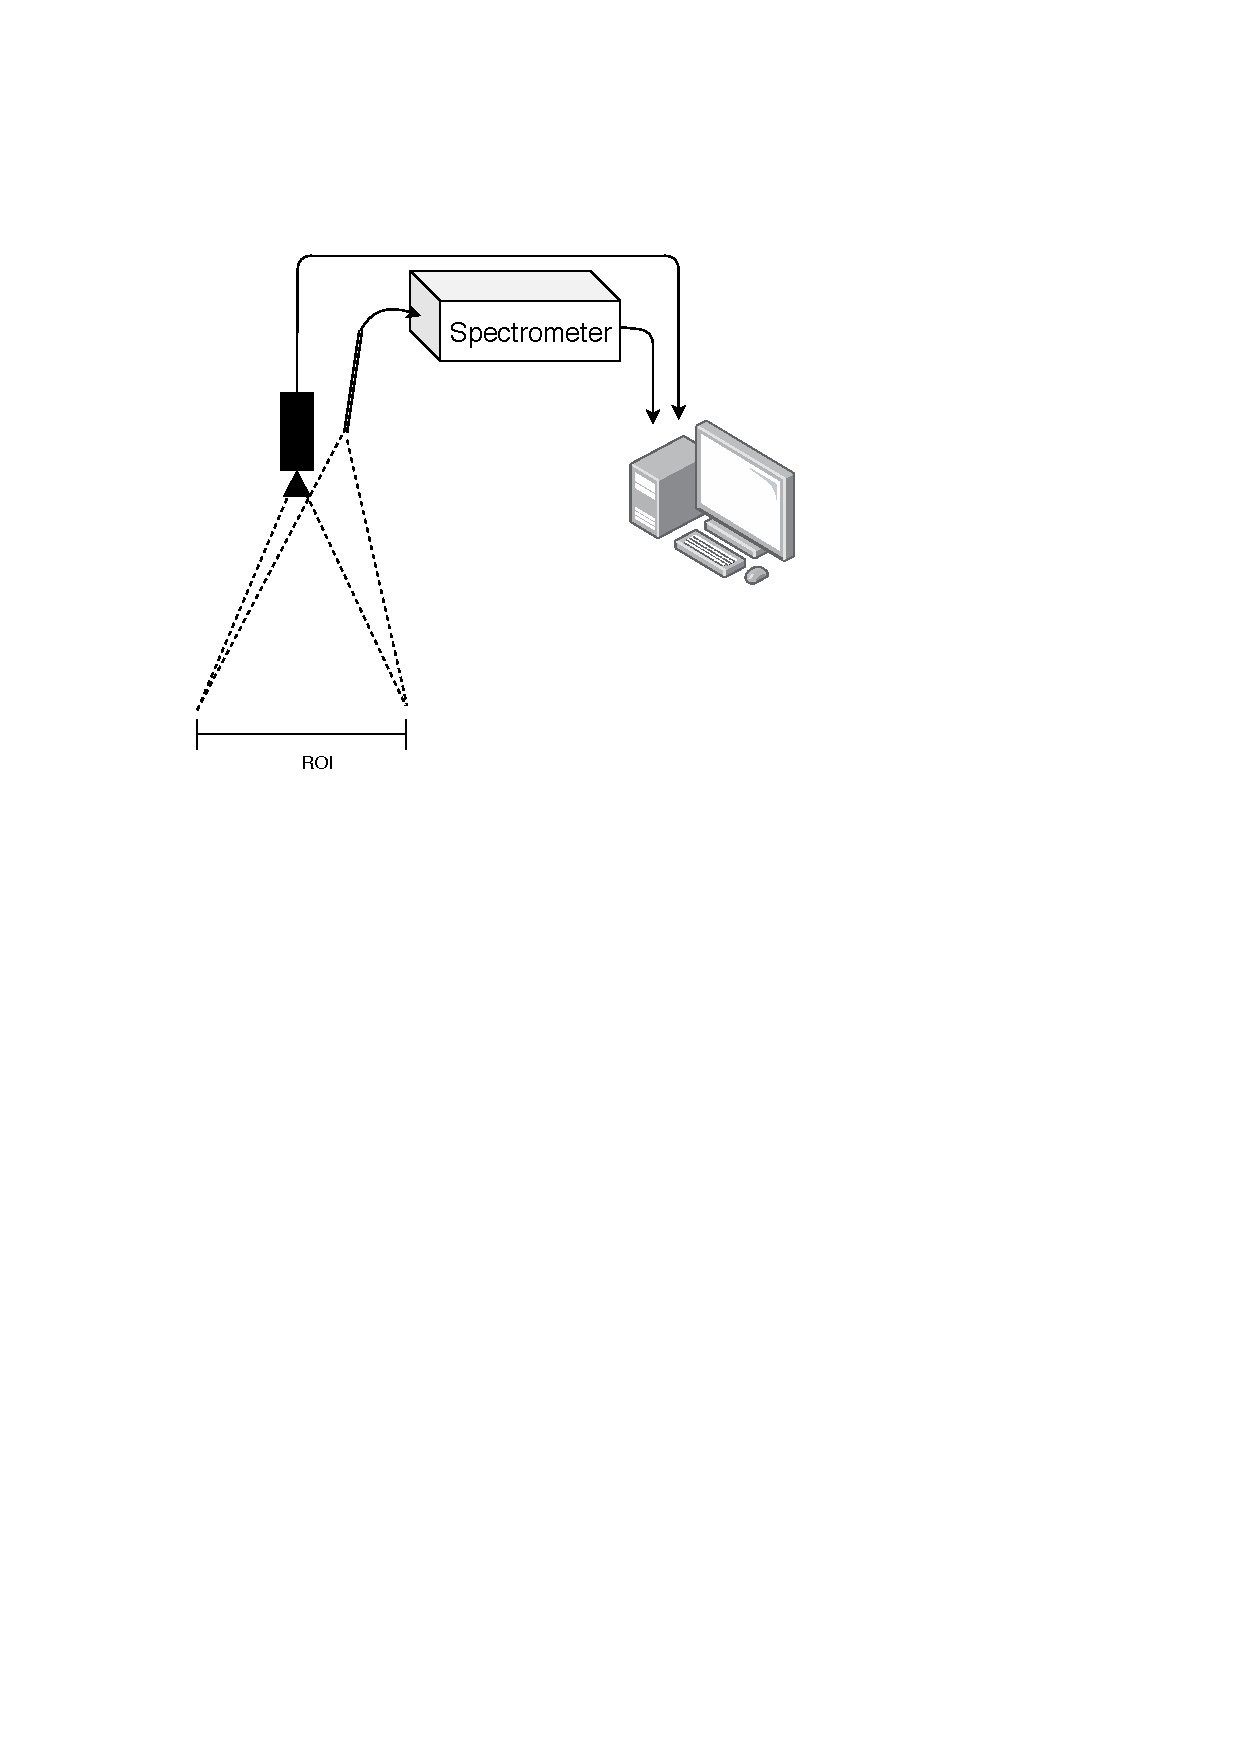
\includegraphics[width=1\textwidth]{figures/pt_setup.pdf}
    \caption{Measurement setup}
    \label{fig:measurement_setup}
\end{figure}

